\documentclass{standalone}
\usepackage{tikz}
\usepackage{ctex,siunitx}
\setCJKmainfont{Noto Serif CJK SC}
\usepackage{tkz-euclide}
\usepackage{amsmath}
\usetikzlibrary{patterns, calc,3d}
\usetikzlibrary {decorations.pathmorphing,decorations.pathreplacing,decorations.shapes}
\begin{document}
\small
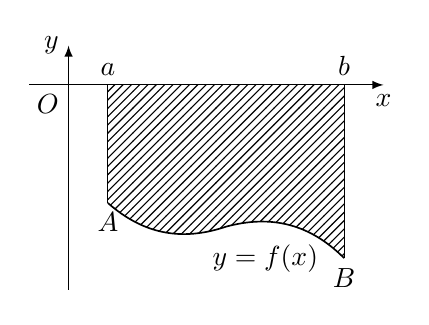
\begin{tikzpicture}[>=latex,scale=1.0]
  \draw[->](-0.5,0)--(4,0)node[below]{$x$};
  \draw[->](0,-2.6)--(0,0.5)node[left]{$y$};
  \node at (0,0)[below left]{$O$};
  \draw[semithick](0.5,-1.5)node[below]{$A$}to[bend right](2,-1.8)to[bend left](3.5,-2.2)node[below]{$B$};
  \draw(0.5,-1.5)--(0.5,0)node[above]{$a$};
  \draw(3.5,-2.2)--(3.5,0)node[above]{$b$};
  \fill[pattern=north east lines](0.5,0)--(0.5,-1.5)to[bend right](2.0,-1.8)to[bend left](3.5,-2.2)--(3.5,0);
  \node at (2.5,-2.2){$y=f(x)$};
\end{tikzpicture}
\end{document}